\documentclass[12pt]{beamer}
\usepackage[utf8]{inputenc} % style d'écriture
\usepackage[T1]{fontenc}      % package
\usepackage[francais]{babel}  % package pour langue française
\usepackage{graphicx}
\usepackage{subcaption}
\usepackage{url}
\usepackage{color}
\usepackage{geometry}
\usepackage{amssymb}

% William PENSEC, étudiant en Master 2 LSE 2020/2021

\usetheme[secheader]{Madrid}
\beamertemplatenavigationsymbolsempty
\setbeamertemplate{frametitle continuation}{}

\title[Compte rendu de stage n\textsuperscript{o}3]{Coopération de drones dans un système hétérogène}
\subtitle{Compte rendu de stage n\textsuperscript{o}3}
\author{William \textsc{Pensec}}
%\author{William \textsc{Pensec}}
%\author{William \textsc{Pensec}}
\institute[Lab-STICC]{Lab-Sticc}
\date{03 mai 2021}

%\AtBeginSection[]
%{
%\begin{frame}<beamer>{Sommaire}
%\tableofcontents[currentsection,currentsubsection, 
%    hideothersubsections, 
%    sectionstyle=show/shaded,
%]
%\end{frame}
%}

\begin{document}
	% ---------------------------------------------------------------- %
	\begin{frame}
		\begin{titlepage}
			\begin{figure}[H]
				\centering
				
\includegraphics[scale=.15]{labsticc.png}
				\hspace{3cm}
				
\includegraphics[scale=.3]{ubo.png}
			\end{figure}
		\end{titlepage}
	\end{frame}
	
	% ---------------------------------------------------------------- %
	\section*{Sommaire}
	\begin{frame}
		\frametitle{Sommaire}
		\begin{center}
			\tableofcontents
		\end{center}
	\end{frame}
	%
	% ---------------------------------------------------------------- %
	\section{Installation OSDK sur Raspberry Pi}	
	\begin{frame}
	\frametitle{\bsc{Installation OSDK sur Raspberry Pi}}
	    \begin{block}{}
			\begin{itemize}
    	    \setbeamertemplate{itemize items}[square]
				\item Tourne sur Raspbian mais fait davantage pour Ubuntu (16.0)
				\item Relié via l'UART du drone et les pins RX/TX du Raspberry
				\item Permettra d'accéder aux capteurs du drone
				\item Permettra de déplacer le drone (décollage et atterissage compris) 
			\end{itemize}
		\end{block}
	\end{frame}	
	%
	% ---------------------------------------------------------------- %
	\section{Communication entre le drone et le Raspberry Pi}	
	\begin{frame}[allowframebreaks]
    	\frametitle{Communication entre le drone et le Raspberry Pi}
    	    \begin{figure}[H]
				\centering
				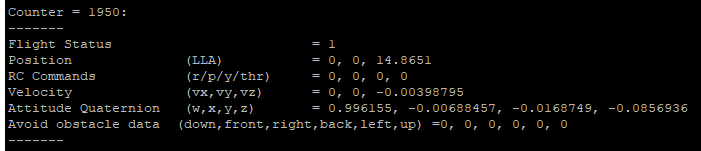
\includegraphics[scale=0.62]{telemetry.png}
			\end{figure}
			\begin{figure}[H]
				\centering
				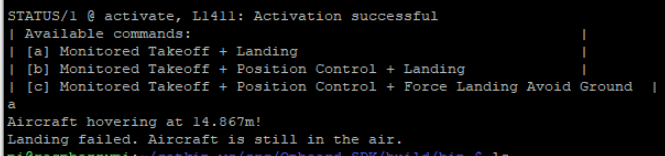
\includegraphics[scale=0.65]{flightcontrol.png}
			\end{figure}
	\end{frame}
	%
	%% ---------------------------------------------------------------- %
	\section{A faire}
	\begin{frame}
	\frametitle{A faire}
	    \begin{alertblock}{}
    	    \begin{itemize}
    	    \setbeamertemplate{itemize items}[triangle]
    	        \item Lecture des données des cartes Decawave (ultra large bande)
    	        \item Positionnement du drone dans la pièce à un moment donné
    	        \item Envoi et réception d'informations au drone via l'UART et le SDK
    	    \end{itemize}
	    \end{alertblock}
	\end{frame}
	%
	% ---------------------------------------------------------------- %
	\section*{Remerciements}
	\begin{frame}
	\frametitle{Remerciements}
		\begin{center}
		Merci pour votre attention!

		\bigbreak
		Avez-vous des questions?
		\end{center}
	\end{frame}
	% ---------------------------------------------------------------- %
	
	%\section*{Bibliographie}
	%\begin{frame}[allowframebreaks]
	%\frametitle{Bibliographie}
		%\bibliographystyle{unsrt}
		%\bibliography{bibliographie}
	%\end{frame}
	% ---------------------------------------------------------------- %
\end{document}